在顺序队列中,{通常让队尾指针rear指向队尾元素,让队首front指针指向队头元素的前一个位置。}(但这不是一定的,如2011年真题的第3道选择,就让front指向了队头元素)

为了预防rear和front都到达数组末端,造成无法让元素进队的情况,就需要把顺序队列改进为循环队列。如何实现指针的循环是一个问题,下面的语句解决了这个问题。

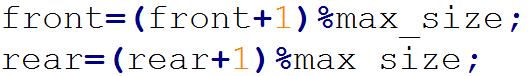
\includegraphics[width=2.39583in,height=0.34375in]{png-jpeg-pics/E027815619E166F3A6DF9E1573525F07.png}

对于循环队列两个特殊的状态,表示如下:

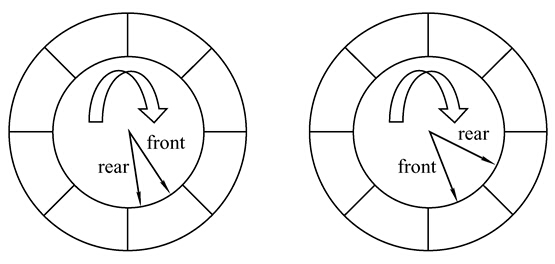
\includegraphics[width=2.08333in,height=2.08333in]{png-jpeg-pics/8616513dd4ea9ae6d81e012612d36a82?}

考生可以自己先猜一下,哪个表示队空,哪个表示队满。

由定义可知,非空位置范围其实是front指针沿顺时针方向到达rear位置,扫过的空间为队列部分。但若front和rear都指向同一位置,就不知道其为空队,还是满队了。{为了区分,循环队列必须损失一个存储空间},如右图的情况,除了front位置,其余都为非空,定为队满的情况。就不能让rear超过front一圈(就好像两个同学在400m跑道上进行长跑一样,考虑到跑慢同学的自尊心,要求跑快的同学rear不可以超过跑慢同学front一圈,即最多超过他399m,就不能再超了)。

综上,左图为队空(rear==front),右图为队满(rear+1)\%max\_size==front。
